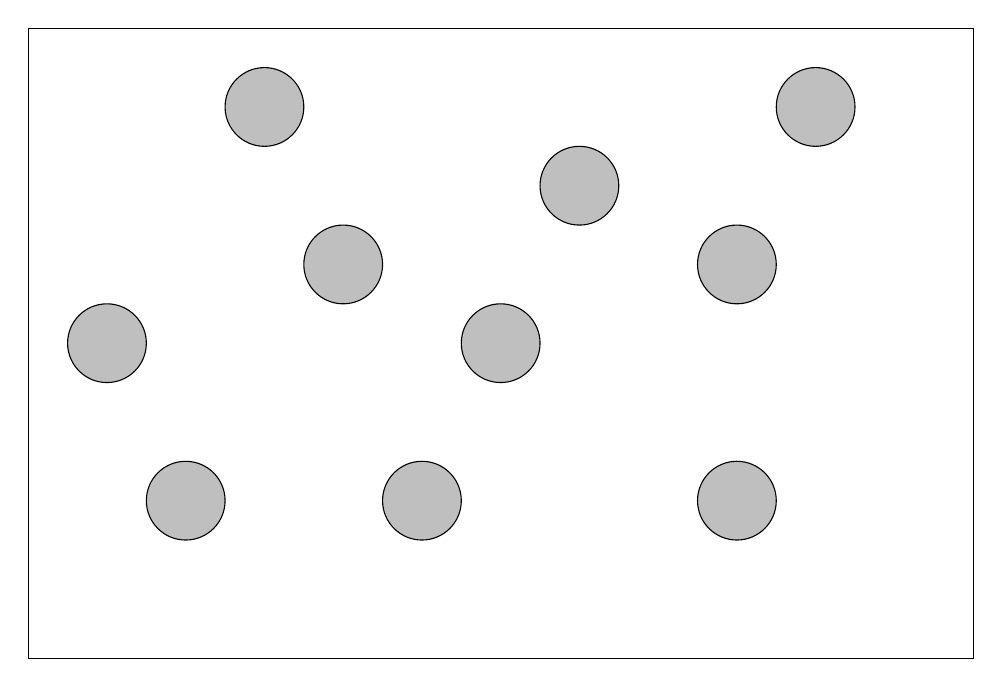
\begin{tikzpicture}

\draw[black] (0,0) -- (0,8) -- (12,8) -- (12,0) -- (0,0);
\filldraw[fill = lightgray, draw = black] (3,7) circle (0.5 cm);
\filldraw[fill = lightgray, draw = black] (1,4) circle (0.5 cm);
\filldraw[fill = lightgray, draw = black] (5,2) circle (0.5 cm);
\filldraw[fill = lightgray, draw = black] (6,4) circle (0.5 cm);
\filldraw[fill = lightgray, draw = black] (9,2) circle (0.5 cm);
\filldraw[fill = lightgray, draw = black] (2,2) circle (0.5 cm);
\filldraw[fill = lightgray, draw = black] (7,6) circle (0.5 cm);
\filldraw[fill = lightgray, draw = black] (4,5) circle (0.5 cm);
\filldraw[fill = lightgray, draw = black] (10,7) circle (0.5 cm);
\filldraw[fill = lightgray, draw = black] (9,5) circle (0.5 cm);
\end{tikzpicture}
\newline

Momentum is important because it describes how objects move in our Newtonian framework. We have written before that $\vec{F} = m\vec{a}$, but this is not quite correct. If you were like me, I am sure you wondered what would happen with force if the mass of the object was changing. Well, as you have probably assumed, it does not follow the fact that $\vec{F}=m\vec{a}$. Nature really follows the fact that \begin{equation}\vec{F}=\frac{d\vec{p}}{dt}\end{equation} Where $\vec{p}$ is momentum. For our purposes, we will define momentum relatively simply, $\vec{p}=m\vec{v}$. It is important to see here that momentum is our vector, just like velocity. This means that laws about momentum must hold in all of the three directions. It is easy to forget this because we will often only look at momentum in a single direction. Nonetheless, it is still important to understand its nature as a vector because more often than not, trick questions surrounding momentum in multiple directions will appear. Looking at momentum's of different objects will allow us to understand what happens during collisions. The examples we will describe may seem fairly contrived, but frankly, the world is made of collisions. Trillions of trillions of particles are hitting each other all the time. Think about air or water, or how any chemical reaction occurs. These things are the result of high-speed particles smashing into each other, sometimes heading their separate ways, and sometimes combining. We will see how to analyze these systems shortly. 